\section{INTRODUCTION}\label{sec:introduction}

Autonomous robots are a promising next step in robotics. They could help solve many of current major societal challenges. Examples include assistance at home\todo[disable]{ref}, in care centres\todo[disable]{ref}, but also in industrial environments~\cite{sup_navigation}.
However, the complicated dynamic environment these robots operate in and the complex actions they have to perform, make this a challenging field. 
Advancements in computing power and hardware have made autonomous robots increasingly capable of providing the complex tasks required to operate in these environments, but at the same time increasingly complex systems.\\ 
Since the introduction of the supervisory control theory of Ramadge and Wonham~\cite{original}, the benefits of supervisory control synthesis have been discussed and proven in numerous papers. Benefits relating to system design, as shown e.g.\@ in~\cite{themepark}, and benefits relating to task execution.
\todo[disable]{ref}

These benefits could help manage the aforementioned increase in complexity in autonomous robotics.\\

Improvements in system design that supervisory control synthesis can offer are illustrated in \cref{fig:TR_and_MB_SE_processes,fig:sup_se} from~\cite{Baeten2016}. 
The figures show the systems engineering design process from traditional to model-based with supervisory control theory included. 
The traditional SE design process and MBSE design process are represented in \cref{fig:TR_and_MB_SE_processes} for a system with a controller \(S\) and plant \(P\).
In traditional SE the requirements are tested on the realization of the design, without using models of the designs.
This is represented in \cref{fig:TR_and_MB_SE_processes} with the \textit{realize} arrow from design to realization.
For complex systems, time-to-market and errors can be reduced by testing the design before realizing it. 
The process of Model Based Systems Engineering (MBSE)~\cite{mbse}, also shown in \cref{fig:TR_and_MB_SE_processes}, uses models of \(S\) and \(P\) for that reason, and, among others,~\cite{themepark} demonstrates that it indeed improves time-to-market and reduces errors.
The next evolution of integrating models in the design process is using supervisory control synthesis of \(S\) from \(P\) and the models of the system requirements (\cref{fig:sup_se}).
Where the traditional SE process relies heavily on documentation, from defining the requirements to realizing a design, the models used in MBSE provide a more systematic and unambiguous specification of \(S\) and \(P\).
This makes working on large multi-disciplinary projects faster and easier.
Finally, using supervisory control synthesis on models of requirements guarantees that requirements are met, even in complex systems.
This reduces the reliance on documentation and testing even more and prevents errors created by the implementation phase of the requirements.\\

\begin{figure}
\begin{center}
\includestandalone[width=0.9\columnwidth]{./images/tikz/Traditional_and_MB_SE}

\scriptsize{
  \tikz[fmbe,baseline=(x.base)]{\node[document] (x) {$\phantom{X}$};} = documents
  \tikz[fmbe,baseline=(x.base)]{\node[model](x){$\phantom{Y}$};} = models
  \tikz[fmbe,baseline=(x.base)]{\node[realization](x){$\phantom{Z}$};} = realizations}
\end{center}
\caption{Traditional and model-based systems engineering processes}
  \label{fig:TR_and_MB_SE_processes}
\end{figure}


\begin{figure}[!h]
  \centering
  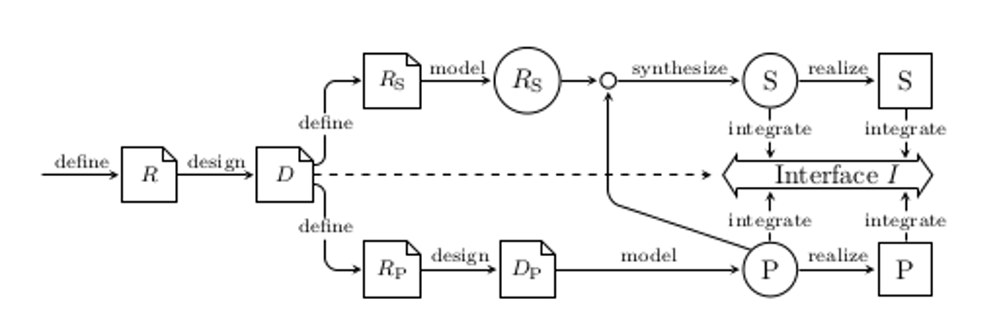
\includegraphics[width=\columnwidth]{sup_se.png}
  \caption{Supervisory control synthesis-based systems engineering process}\label{fig:sup_se}
\end{figure}
\newpage
Besides the above mentioned benefits relating to system design, supervisory control synthesis offers benefits in task execution as well.
Task execution benefits, in this paper, are a group of benefits relating to reductions in man-made errors when programming the robot.
The following guarantees supervisory synthesis offers, would have to be ensured by proper implementation of logic throughout the code, when not using supervisory control synthesis.
This approach, without using supervisory control synthesis, is sensitive to mistakes; incorrectly implementing the logic in just one place can cause unwanted behaviour.
Also, when the system changes, the logic has to be changed everywhere.
Supervisory control theory guarantees synthesis of a non-blocking, maximally permissive and controllable supervisor, as explained in \cref{sec:supervisory_control}.
These are useful when executing tasks, because it removes the ownership of these problems from the software developer to the supervisor.
Another benefit provided by supervisory control synthesis, somewhat specific to this paper, is the more straightforward implementation of concurrent task execution.
Traditionally, the software developer has to implement all the conditions regarding when a task can be executed, has to be interrupted or stopped, himself.
With supervisory control synthesis, however, the supervisor will block all tasks (or events) that violate the requirements.
Therefore, ensuring a task will never be executed untimely, as long as the requirements are specified correctly.\\

Despite the advantages of applying supervisory control theory to autonomous robots, there has been little research in the field. 
The research that has been done usually focusses on using supervisory control to govern the way robots interact with each other~\cite{sup_swarm}, using a human as supervisor~\cite{sup_human} or an autonomous robot operating in a relatively static environment~\cite{sup_navigation}.
This is understandable, because supervisory control has three limitations that seem to make it unsuitable for autonomous robots:

\begin{itemize}
  \item Supervisory control can only be applied to discrete-event systems.
  \item The synthesis of the supervisor is done off-line, so it cannot deal with the robot entering an unknown environment.
  \item Supervisory control theory assumes asynchronous and instantaneous task execution.
\end{itemize}

The purpose of this paper is to investigate these limitations, defining on what abstraction levels supervisory control synthesis can be applied, defined as the application scope, in autonomous robots and to explore the impact and benefits it can have.
Using the Amigo robot at the Eindhoven University of Technology, two case studies are presented. 
These case studies showcase the benefits of using supervisory control synthesis and the application scope of the theory to autonomous robotics. 
A method is proposed that not only presents a new beneficial way to control autonomous robots, but also show what is and what is not (yet) possible.\\

The paper is structured as follows. \Cref{sec:supervisory_control} provides some necessary background on supervisory control theory and discrete-event systems. It is followed by an explanation of the case studies in \cref{sec:case_studies}. The methodology and design choices are explained in \cref{sec:method}.
The results of applying the described method to these case studies are presented in \cref{sec:results}.
Finally, \cref{sec:conclusions} discusses the limitations of using supervisory control synthesis for autonomous robots and possible research that can eliminate them.\\